\chapter{Technische Unterschiede zwischen Xamarin.Forms und Flutter}
\label{chap:CrossPlattformFrameworks}

Die Unterschiede zwischen den Frameworks werden im folgenden genauer betrachtet.  Für den technischen Vergleich dient Xamarin.Forms als Grundlage.  Die Namen von Abschnitten und Unterabschnitten orientieren sich deshalb an dessen Terminologie.  In den jeweiligen Gliederungspunkten wird anschließend genauer betrachtet,  wie sich spezielle Arbeitsweisen oder Darstellungsoptionen in Flutter abbilden lassen. 

\section{Projektaufbau}
Xamarin.Forms weißt eine andere Projektstruktur auf als Flutter,  das nur mit einem Projekt arbeitet.  Wärend das Flutter Projekt alle notwendigen Inhalte für iOS und Android inkludiert, \footcite[Vgl.][S. 113]{Biessek2019} setzt sich die Projektmappe bei Xamarin.Forms aus mehreren Projekten zusammen.  Es gibt für jede Plattform ein dediziertes Projekt, dass den plattformspezifischen Code,  Konfigurationen und Icons beinhaltet, sowie ein Projekt für den plattformunabhängigen Quelltext.   \footcite[Vgl.][S. 25f.]{Petzold2016} Icons und Konfigurationen werden bei Flutter in einem gleichen oder ähnlichen Format und nur in einem anderen Projekt hinterlegt und lassen sich folglich migrieren.  In den Ausschlusskriterien in Kapitel \ref{chap:CompilerEntwurf} dieser Arbeit wurde bereits der plattformspezifische Quelltext von Xamarin.Forms für die Übersetzung exkludiert.  
\section{Ansichten}
Ansichten (engl. Views) sind visuelle Elemente, die in zwei Kategorien unterschieden werden können.  Steuerelemente (engl. Controls) sind für die Sammlung von Benutzereingaben oder die Ausgabe von Daten verantwortlich und Layouts, beinhalten eine Sammlung von Ansichten und sind für ihre visuelle Anordung auf der Benutzeroberfläche verantwortlich.  \footcite[Vgl.][Abgerufen am \today]{Ritscher2020}

\subsection{Layouts}
Ähnlich wie die Ansichten lassen sich auch die Layouts in zwei Kategorien unterteilen.  Den Ansichtsseiten (engl. Pages) sowie den generellen Layouts. 
Die Pages nehmen den gesamten Bildschirm ein und werden in Abbildung \ref{fig:Xamarin.Forms Pages} dargestellt.\footcite[Vgl.][Abgerufen am \today]{MicrosoftXamPages2016}  

\begin{figure}[!ht]
 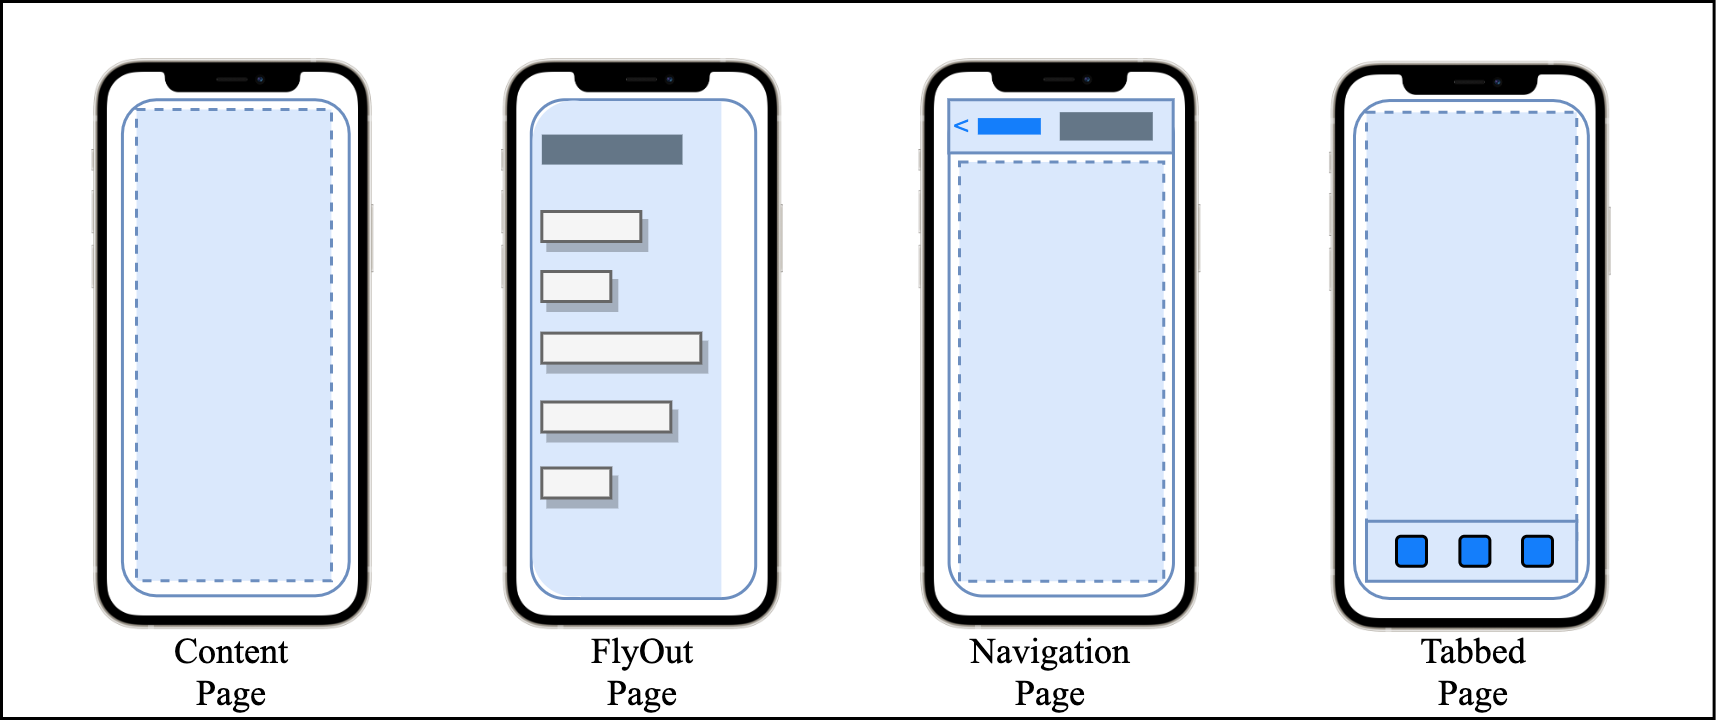
\includegraphics[width=\textwidth,height=\textheight,keepaspectratio]{Images/CrossPlattformFrameworks/XamarinFormsPages.png}
 \caption[Xamarin.Forms Pages]{Xamarin.Forms Pages\footcite{MicrosoftXamPages2016}}
 \label{fig:Xamarin.Forms Pages}
\end{figure}

\glq ContentPage \grq{} ist ausschließlich für die Anzeige einer weiteren Ansicht verantwortlich.  Die drei anderen Pages besitzen ein Navigationskonzept.  \footcitetext[Abbildung in Anlehnung an ][Abgerufen am \today]{MicrosoftXamPages2016} \glq FlyOutPage\grq{} teilt den Bildschirm in zwei Bereiche, ein Bereich dient der Navigation.  Er enthält ein Menü das wie im Namen enthalten einfliegen kann.  Der zweite Bereich zeigt eine Detailansicht,  in welcher der Inhalt der angeforderten Seite geladen wird.  \glq NavigationPage\grq{} bietet eine Navigationsleiste, die einen Titel der aktuellen Seite und eine Navigationsschaltfläche beinhalten kann.  \glq TabbedPage\grq{} stellt die unterschiedlichen Seiten als Registerkarten dar. \footcite[Vgl.][Abgerufen am \today]{MicrosoftXamPages2016}
Die Ansichtseiten befinden sich in der Regel, innerhalb der XAML-Datei, auf der untersten Ebene, dem so genannten Wurzelknoten. Der Quelltext \ref{lst:TabbedPage} zeigt dies exemplarisch für eine \glq TabbedPage\grq{} dargestellt,  angegeben.  

\lstinputlisting[label={lst:TabbedPage},caption={[Xamarin.Forms \glq TabbedPage\grq{} Definition]{Xamarin.Forms \glq TabbedPage\grq{} Definition\footcite[Quelltext in Anlehnung an][Abgerufen am \today]{MicrosoftXamTabbedView2020}}} , language=XML]{SourceCode/XamarinFormsTabbedPage.XAML}

Es wird eine \glq TabbedPage\grq{} mit drei Registerkarten entworfen.  Eine Kombination mehrerer Navigationskonzepte ist hier wie das Beispiel zeigt möglich,  hier befindet sich eine Navigationsleiste innerhalb der Registerkarten. 

Die verfügbaren Eigenschaften der Ansichtsseiten unterscheiden sich je nach Einsatzszenario.  Im folgenden Quelltext \ref{lst:FlyOutPage} wird dies am Beispiel der Realisierung einer \glq FlyoutPage\grq deutlich.  Anders als bei \glq TabbedPage\grq{}  die aus einer Sammlung von Registerkarten besteht finden sich an dieser Stelle die Eigenschaften \glq Flyout\grq{}  und \glq Detail\grq{}.

\lstinputlisting[label={lst:FlyOutPage}, caption={[Xamarin.Forms \glq FlyoutPage \grq{} Definition]{Xamarin.Forms \glq FlyoutPage\grq{} Definition\footcite[Quelltext in Anlehnung an][Abgerufen am \today]{MicrosoftXamFlyOutPage2020}}} ,language=XML]{SourceCode/XamarinFormsFlyoutPage.XAML}

Im Unterschied zu Xamarin.Forms lässt kann Flutter auf der Wurzelebene nur den Style der App nicht aber ein Navigationskonzept definieren.  Wie bereits in Kapitel \ref{chap:CompilerEntwurf} aufgeführt, wird in dieser Arbeit ausschließlich der Material Design Style unterstützt. \footcite[Vgl.][Abgerufen am \today]{FlutterForXFDevs} Quelltext \ref{lst:MaterialApp} zeigt die Realisierung einer MaterialDesign App in Flutter.
\newpage
\lstinputlisting[label={lst:MaterialApp}, caption={[Flutter \glq MaterialApp\grq{} Definition]{Flutter \glq MaterialApp\grq{} Definition\footcite[Quelltext in Anlehnung an][Abgerufen am \today]{GoogleFlutterFirstApp2020}}}, language=Dart]{SourceCode/MaterialApp.Dart}

Der Vergleich zwischen den Extensible Markup Language(XML) basierten XAML-Dateien und den bei Flutter verwendeten Dart-Dateien verdeutlicht die Unterschiede in den verwendeten Sprachen zur Benutzeroberflächen Entwicklung. 

Die zentrale Idee hinter dem Flutter-Framework ist es,  eine Benutzeroberfläche aus Widgets aufzubauen.  Diese beschreiben das Aussehen der Anwendung basierend auf ihrem aktuellen Zustand.  Sobald er sich ändert, kann das Framework den neuen mit dem alten Status vergleichen, um grafische Veränderungen möglichst effektiv vorzunehmen. \footcite[Vgl.][Abgerufen am \today]{GoogleWidgets2020}  Damit in Flutter ein Navigationskonzept definiert werden kann,  können verschiedene  Widgets verwendet und verschachtelt werden,  dies wird in Quelltext \ref{lst:FlutterTabbedApp} exemplarisch für eine App mit Registerkarten visualisiert.

\lstinputlisting[label={lst:FlutterTabbedApp},caption={[Flutter \glq Tab Layout\grq{} Definition]{Flutter \glq Tab Layout\grq{} Definition\footcite[Quelltext in Anlehnung an][Abgerufen am \today]{GoogleFlutterTabs2020}}}, language=Dart]{SourceCode/TabbedPage.Dart}

Die deutliche Unterschiede bei der Auswahl eines Navigationkonzeptes können dadurch überbrückt werden, dass man zu jeder Xamarin.Forms Page das entsprechende Flutter Widget findet.  Der Flutter-Widgetkatalog\footcite[Vgl.][Abgerufen am \today]{GoogleFlutterWidgetCatalog2020} und die Webseite "Flutter for Xamarin.Forms Developers"\footcite[Vgl.][Abgerufen am \today]{FlutterForXFDevs} wurde für die Recherche des Gegenstückes verwendet.  Entsprechende Ergebnisse der Suche können in Tabelle \ref{tab:ComapreXFFlutter} abgelesen werden. 


\begin{table}[!ht]
\begin{tabularx}{\textwidth}{X|X}
   \textbf{Xamarin.Forms Page} & \textbf{Flutter Widget}  \\
\hline
	ContentPage            &           	\\ 
	FlyOutPage             & MasterDetailScaffold          	\\ 
	NavigationPage       & Scaffold         	 					\\ 
	TabbedPage            & TabBar und TabBarView 		\\ 
\end{tabularx}
\caption{Gegenüberstellung Pages}
 \label{tab:ComapreXFFlutter}
\end{table}
Diese Gegenüberstellung,  in Tabellenform,  von Xamarin.Forms Elementen und Flutter Widgets wird auch an anderer Stelle in diesem Kapitel der Übersichtlichkeit halber verwendet.  Eine vollständige Referenztabelle die sich aus allen Einzelbetrachtungen zusammensetzt befindet sich in Anhang X. 


Neben den Ansichtsseiten bietet Xamarin.Forms jedoch weitere Layouts,  die Steuerelemente zu visuellen Strukturen zusammenstellen.  Abbildung \ref{fig:Xamarin.Forms Layouts} visualisiert die wichtigsten dieser Layouts. 

\begin{figure}[!ht]
 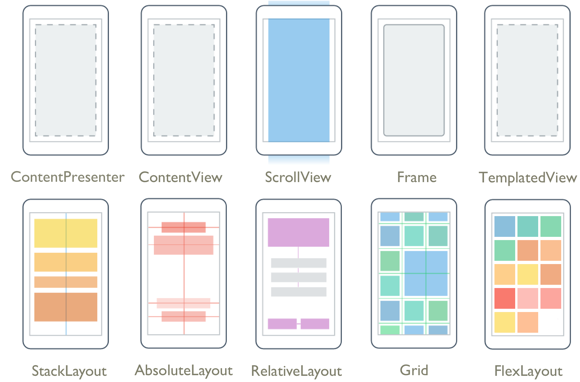
\includegraphics[width=\textwidth,height=\textheight,keepaspectratio]{Images/CrossPlattformFrameworks/XamarinFormsLayouts.png}
 \caption[Xamarin.Forms Layouts]{Xamarin.Forms Layouts\footcite{MicrosoftXamViews2020}}
 \label{fig:Xamarin.Forms Layouts}
\end{figure}

Die in der Abbildungen visualisierten Layouts werden innerhalb von Xamarin.Forms Anwendungen am häufigsten benutzt und haben haben die folgenden visuellen Eigenschaften.  \footcitetext[Abbildung in Anlehnung an ][Abgerufen am \today]{MicrosoftXamLayouts2018} \glq ContentView\grq{}  enthält ein einzelnes untergeordnetes Ansichtselement und wird als Basisklassen für eigene Darstellungen verwendet.  Ein \glq StackLayout\grq{}  positioniert die untergeordnete Elemente in einem Stapel entweder horizontal oder vertikal.  Ein \glq Grid\grq{}  positioniert seine untergeordneten Elemente in einem Raster aus Zeilen und Spalten,  es wird aber auch häufig für die visuelle Stapelung von Layouts und Steuerelementen verwendet.  Das \glq ScrollView\grq{} erlaubt es seinen Inhalt, wie der Name es vermuten lässt,  zu scrollen. Neben diesen häufig verwendeten Layouts gibt es noch weitere die jedoch nicht so häufig verwendet werden.  Dazu gehört ein Frame, welches einen Rahmen um ein visuelles Element zeichnet.  Das AbsolutLayout, welches untergeordnete Elemente an bestimmten Positionen relativ zu ihrem übergeordneten Element plaziert und das RelativeLayout welches die gleiche Aufgabe relativ zum RelativLayout oder seiner Kinder übernimmt.\footcite[Vgl.][Abgerufen am \today]{MicrosoftXamLayouts2018}

Basierend auf diesen Verfügbaren Layouts werden in Tabelle \ref{tab:XamLayouts}  die es entsprechende Flutter Widgets aufgeführt.  Diese wurden wie die Ansichtsseiten mit dem Flutter Widget Katalog erarbeitet.  Teilweise haben diese Widgets jedoch auch erweitere Funktionalitäten.  So muss für die Verwendung eines scrollbaren \glq Grids in Xamarin.Forms dieses in einer \glq ScrollView\grq{}  hinterlegt werden. In Flutter ist bietet das \glq GridView\grq{}  Widget diese von sich aus an,  wenn der Inhalt den sichtbaren Bereich überschreitet. \footcite[Vgl.][Abgerufen am \today]{GoogleFlutterGridView2020} Dies hat zur Folge,  innerhalb der Codeoptimierung des Compilers \glq ScrollViews\grq{}  um \glq Grids\grq{}  entfernt werden könnnen. 

\begin{table}[!ht]
\begin{tabularx}{\textwidth}{X|X}
   \textbf{Xamarin.Forms Page} & \textbf{Flutter Widget}  \\
\hline
	AbsolutLayout       		&  Positioned	 			\\ 
	ContentView       		&  StatelessWidget	 			\\ 
	Frame       					&  BoxDecoration     	 			\\ 
	Grid            				&  GridView oder Stack für das Stapeln von Elementen						\\ 
	ScrollView            		&  SingleChildScrollView		\\ 
	StackLayout       		&  Row und Column  	 			\\ 
	ReleativLayout           &  Positioned		\\ 

\end{tabularx}
\caption{Gegenüberstellung Layouts}
 \label{tab:XamLayouts}
\end{table}

\subsection{Steuerelemente}

Steuerelemente sind die Bausteine der Benutzeroberflächen in Xamarin.Forms, zu Ihnen gehören zum Beispiel Schaltflächen, Beschriftungen und Textfelder.  Xamarin.forms kategorisiert Steuerelemente innerhalb der Dokumentation anhand ihrer Hauptaufgaben,  der Übersichtlichkeit halber wird diese Kategorisierung in diesem Abschnitt übernommen.  \footcite[Vgl.][Abgerufen am \today]{MicrosoftXamViews2020}

\subsubsection{Steuerelemente zur Darstellung}
Diese Steuerelemente sind Ausschließlich für die Darstellung von Inhalten vorgesehen,  klassischerweise sind dies Informationen die für die Arbeit mit der Anwendung wichtig sind an.  Im folgenden werden die wichtigsten Steuerelemente dieser Kategorie vorgestellt,  wobei zu zeichnende Elemente wie die \glq Ellipse\grq{} ,  \glq Linie\grq{} , \glq Path\grq{} ,  \glq Polygon,\grq{}   \glq Polyline\grq{}  und \glq Rectangle\grq{}  nicht besonders aufgeführt werden,  da diese bei Flutter einfach auf die sogenannte Canvas gezeichnet werden können.  \footcite[Vgl.][Abgerufen am \today]{GoogleFlutterCanvas2020} In Xamarin. Forms gibt es die folgenden Darstellungssteuerelemente für die eine Flutter Repräsentation notwendig ist.  Das Steuerelement \glq BoxView zeigt in Xamarin.Forms ein einfarbiges Rechteck an. Häufig wird eine \glq BoxView\grq{}  jedoch auch dafür benutzt einen Strich als Separator zwischen anderen visuellen Elementen darzustellen.  Für die Darstellung von Texten wird in Xamarin.Forms auf \glq Label\grq{} zurückgegriffen. Bilder können mit Hilfe des \glq Image\grq{}  Steuerelement geladen werden,  wobei die Bilder aus verschiedenen Quellen geladen werden können.  Dazu gehören das Web oder aus den Ressourcen der App.  Das Steuerelement \glq Map\grq{}  kann für die Anzeige von Karten innerhalb der App verwendet werden.  Zur Darstellung von Webseiten und Hypertext Markup Language (HTML) Dokumenten kann das \glq WebView\grq{}  Steuerelement verwendet werden.  \footcite[Vgl.][Abgerufen am \today]{MicrosoftXamLayouts2018} Für die Steuerelemente kann nun eine Gegenüberstellung zwischen Xamarin.Forms Pages und Flutter Widgets vorgenommen werden dies wird in Tabelle \ref{tab:ControlsVisualization} dargestellt.


\begin{table}[!ht]
\begin{tabularx}{\textwidth}{X|X}
   \textbf{Xamarin.Forms Page} & \textbf{Flutter Widget}  \\
\hline
	BoxView		       			&   	 SizedBox oder 	Divider 		\\ 
	Image       						&	     Image	 			\\ 
	Label       						&  	Text oder RichText 			\\ 
	Map            					&	   	Leamaps oder Google Maps \\ 
	WebView            			&  	webview\_flutter	\\ 
	Ellipse							&  	CustomPaint	\\ 
	Linie								&	  	CustomPaint	\\ 
	Path  							&  	CustomPaint	\\ 
	Polygon  						&  	CustomPaint	\\ 
	Polyline und Rectangle  &  	CustomPaint	\\ 
	Rectangle  					&  	CustomPaint	\\ 

\end{tabularx}
\caption{Gegenüberstellung Darstellungssteuerelemente}
 \label{tab:ControlsVisualization}
\end{table}

\subsubsection{Ereignisauslösende  Steuerelemente}
Xamarin.Forms ist ein ereignisgesteuertes Framework,  die hier behandelten Steuerelemente stellen alle mindestens ein Ereignissen zur Verfügung,  das mithilfe von Codebehind Klassen abonniert werden können.  Auf diese Art und Weise wird die Codebehind Klasse informiert, sobald dieses Ereignis ausgelöst wird.  Die meisten dieser Ereignisse werden dabei von Steuerelementen ausgelöst, wenn mithilfe von Gesten mit ihnen interagiert wurde.  Die folgenden Steuerelemente lösen dabei die folgenden Ereignisse aus.  \glq Buttons\grq{}  sind ein rechteckiges Objekt,  die ein \glq clicked\grq{}  Event auslösen nachdem es von einem Anwender gedrückt wurde. Ähnlich funktioniert das \glq ImageButton\grq{}  Steuerelement das als Unterschied statt einem Text ein Icon anzeigt.  Bei einem \glq RadioButton\grq{}  wird eine Option aus einer Menge von Möglichkeiten ausgewählt und löst ein \glq CheckedChanged\grq{}  Ereignis aus, wenn die Auswahl geändert wird.  Das \glq RefreshView\grq{}  ist ebenfalls als Layout-Element, dass eine \glq PullToRefresh\grq{}  funktionalität für scrollbare Inhalte anbietet und ein Event auslöst, wenn diese Interaktion durchführt wurde.  Die \glq Searchbar\grq{}  ist eine Suchleiste, über die der Benutzer Textzeichenfolgen eingeben kann und per Schaltfläche, oder Tastaturtaste,  kann \glq Searched-Event\grq{} ausgelöst werden.  Ein \glq Swipeview\grq{}  ist evenfalls ein Container Steuerelement, welches durch Wischgesten ein Kontextmenü zur Verfügung stellt. 
Tabelle \ref{tab:ControlsVisualization} zeigt die Steuerelemente und Ihre Gegenstücke aus dem Flutter Framework. 
\begin{table}[!ht]
\begin{tabularx}{\textwidth}{X|X}
   \textbf{Xamarin.Forms Page} & \textbf{Flutter Widget}  \\
\hline
	Button		       				&  	Flatbutton 		\\ 
	ImageButton		       		&  	IconButton 		\\ 
	RadioButton		       		&  	RadioButton 		\\ 
	RefreshView		       		&  	pull\_to\_refresh 		\\ 
	SearchBar		       			&  	flutter\_search\_bar 	\\ 
	SwipeView		       		&  	flutter\_slideable 		\\ 
\end{tabularx}
\caption{Gegenüberstellung ereignisauslösende Steuerelemente}
 \label{tab:eventcommands}
\end{table}

Nicht alle Steuerelemente verhalten sich immer exakt gleich wie die Xamarin.Forms Steuerelemente. Ein Beispiel ist die hier erwähnte SearchBar, die bei Flutter im Gegensatz zu Xamarin.Forms nicht frei plazierbar ist, sondern immer in der Navigationsleiste angezeigt wird.  Alternativ wäre es jedoch auch möglich,  das gliche Verhalten mit einem Textinput Feld zu generieren die anliegend beschrieben werden. 


\subsubsection{Wertsetztende Steuerelemente}

Steuerelemente die Werte setzen sind User Interface Elemente die von einem Anwender durch Interaktion mit Werten versehen werden können um diese in der Anwendung zu verarbeiten.  In diesem Unterabschnitt wird nicht auf Elemente eingegangen,  die zur Eingabe und Manipulation von Texten zur Verfügung stehen, da diesen Steuerelementen ein eigener Unterabschnitt gewährt wird.  Xamarin.Forms bietet eine Vielzahl von Steuerelementen, die an dieser Stelle aufgeführt werden. Zusätzlich wird wie in den vorherigen Abschnitten erläutert, wie dieses Verhalten bei Flutter generiert werden kann. 
\begin{itemize}

\begin{table}[!ht]
\begin{tabularx}{\textwidth}{X|X}
   \textbf{Xamarin.Forms Page} & \textbf{Flutter Widget}  \\
\hline
	CheckBox		       				&  	 		\\ 
	Switch		       					&  	 		\\ 
	Slider		       					&  	 		\\ 
	Stepper		       				&  	 		\\ 
	DatePicker		       			&  			\\ 
	TimePicker		       			&  	 		\\ 
\end{tabularx}
\caption{Gegenüberstellung wertsetzender Steuerelemente}
 \label{tab:eventcommands}
\end{table}

\setlength\itemsep{-0.6em}
 \item CheckBox ermöglicht dem Benutzer die Auswahl eines booleschen Wertes mit Hilfe einer Art Schaltfläche, die entweder markiert oder leer sein kann. Flutter bietet ebenfalls ein Checkbox Control an,  das Material Design Checkbox. 
  \item Switch hat die Form eines Ein/Aus-Schalters, damit der Benutzer einen booleschen Wert auswählen kann, für das es ebenfalls eine entsprechendes Flutter Widget gibt. 
 \item Slider bieten Benutzern die Option einen  Wert aus einem kontinuierlichen Bereich auswählen, der mit den Eigenschaften Minimum und Maximum festgelegt wurde.  Flutter bietet ebenfalls ein Widget für Slider an
 \item Stepper ermöglicht es dem Benutzer, einen doppelten Wert aus einem Bereich von inkrementellen Werten auszuwählen, die mit den Eigenschaften Minimum, Maximum und Inkrement festgelegt wurden.  Von Haus aus gibt es bei Flutter kein Steuerelement,  welches ähnliche Eigenschaften anbietet.  Die Open Source Community hat mit dem number\_inc\_dec Plugin aber eine Widget entwickelt welches wie die Xamarin.Forms alternative arbeitet. 
 \item DatePicker ermöglicht es dem Benutzer, ein Datum mit der Datumsauswahl der Plattform auszuwählen.  In Flutter stehen dafür kein Widget sondern eine Funktion zur Verfügung,  die klassischerweise, wie in Quelltext , in einem Gesture Detector auf einem anderen Widget ausgeführt wird.  
 \item TimePicker ermöglicht dem Benutzer die Auswahl einer Zeit mit dem spezifischen TimePicker der Plattform.  Wird ähnlich wie der Datepicker nicht als Widget sonders als Funktionalität ausgeliefert,  ein mögliche Definition ist in Quelltext \ref{lst:FlutterTimePicker} dargestellt.
 
 \begin{minipage}{\linewidth}
\lstinputlisting[label={lst:FlutterTimePicker},caption={Verwendung von Timepickern in Flutter}, language=Dart]{SourceCode/FlutterTimePicker.Dart}
\end{minipage}

\end{itemize}

\subsubsection{Steuerelemente um Text zu manipulieren}
Wie bereits im vorherigen Abschnitt beschrieben sind Steuerelemente zur Eingabe und manipulation von Texten Strang genommen ebenfalls Steuerelemente zum setzen von Werten.  In Xamarin Forms stehen die folgenden beiden Steuerelemente für die Arbeit mit Texten zur Verfügung:
\begin{itemize}
\setlength\itemsep{-0.6em}
 \item Entry ermöglicht dem Benutzer die Eingabe und Bearbeitung einer einzelnen Textzeile., optional kann dieses als Passworteingabe mit Sternen maskiert werden.
 \item Editor ermöglicht dem Benutzer die Eingabe und Bearbeitung mehrerer Textzeilen
\end{itemize}

\begin{table}[!ht]
\begin{tabularx}{\textwidth}{X|X}
   \textbf{Xamarin.Forms Page} & \textbf{Flutter Widget}  \\
\hline
	Entry		       		&  	 		\\ 
	Editor		       	&  	 		\\ 
\end{tabularx}
\caption{Gegenüberstellung textmanipulierender Steuerelemente}
 \label{tab:eventcommands}
\end{table}


In flutter gibt es ausschließlich das Textfield Widget, welches die Funktionalitäten von beiden Xamarin.Forms controlls bündelt.  Standardmäßig bietet das TextField Widget die Eingabemöglichkeit für eine Zeile ähnlich wie das Entry Steuerelement kann aber durch die Eigenschaft "keyboardType: TextInputType.multiline" wie ein entry fungieren wobei optional auch eine Anzahl von maximalen Zeilen übergeben werden kann.  Dies wird in Quelltext dargestellt.

 \begin{minipage}{\linewidth}
\lstinputlisting[label={lst:FlutterTextField},caption={TextField mit mehreren Zeilen in Flutter}, language=Dart]{SourceCode/FlutterTextField.Dart}
\end{minipage}


\subsubsection{Steuerelemente um eine Aktivität anzudeuten}

In mobilen Anwendungen kann es aufgrund der Limitierten Hardware Ressourcen und der begrenzten Netzwerkanbindung dazu kommen, dass Aktionen etwas länger dauern,  als es der Anwender erwarten würden.  Dafür stehen in Xamarin.Forms Steuerelemente zur Verfügung, die dem Anwender das Andauern einer Aktivität andeuten.  Die folgenden Elemente stehen Xamarin.Forms Entwicklern zur Verfügung:

\begin{itemize}
\setlength\itemsep{-0.6em}
 \item ActivityIndicator verwendet eine Animation, um zu zeigen, dass die Anwendung eine langwierige Aktivität ausführt, ohne einen Hinweis auf den Fortschritt zu geben.  Für Flutter Anwendungen steht ein ähnliches Widget zur Verfügung das als "CircularProgressIndicator" bezeichnet wird. 
 \item ProgressBar verwendet eine Animation, um zu zeigen, dass die Anwendung durch eine langwierige Aktivität fortschreitet. In Flutter steht mit dem "LinearProgressIndicator" Widget ebenfalls eine Progressbar zur Verfügung.
\end{itemize}

\begin{table}[!ht]
\begin{tabularx}{\textwidth}{X|X}
   \textbf{Xamarin.Forms Page} & \textbf{Flutter Widget}  \\
\hline
	ActivityIndicator		       		&  	 		\\ 
	ProgressBar		       				&  	 		\\ 
\end{tabularx}
\caption{Gegenüberstellung aktivitätsandeutender Steuerelemente}
 \label{tab:eventcommands}
\end{table}


\subsubsection{Steuerelemente um Sammlungen anzuzeigen}

Bei diesen Steuerelementen handelt es sich um Elemente, die zur Anzeige von Daten-Sammlungen spezialisiert sind.  Xamarin.Forms stellt die folgenden Steuelemente zur Verfügung.


\begin{table}[!ht]
\begin{tabularx}{\textwidth}{X|X}
   \textbf{Xamarin.Forms Page} & \textbf{Flutter Widget}  \\
\hline
	CarouselView		       		&  	 		\\ 
	IndicatorView		       		&  	 		\\ 	
	Picker		       					&  	 		\\ 
	TableView		       				&  	 		\\ 
\end{tabularx}
\caption{Gegenüberstellung sammlungsanzeigender Steuerelemente}
 \label{tab:eventcommands}
\end{table}


\begin{itemize}
\setlength\itemsep{-0.6em}
 \item CarouselView zeigt eine blätterbare Liste von Datenelementen an.  Für Flutter steht ein ähnliches Widget mit dem "carousel\_slider" zur erfügung
 \item IndicatorView zeigt Indikatoren an, die die Anzahl der Elemente in einer CarouselView darstellen
 \item Picker zeigt ein ausgewähltes Element aus einer Liste von Textzeichenfolgen an und ermöglicht die Auswahl dieses Elements, wenn die Ansicht angetippt wird.  Das Picker Widget ist bereits wie im Date,- und Time-Picker beschrieben kein Controll sondern eine Funktion, welches durch Gesten auf andere Widges ausgeführt werden kann. 
 \item TableView zeigt eine Liste von Zeilen mit optionalen Überschriften und Unterüberschriften an.  Das äquivalente flutter- Widget ist als Table Verfügbar.
\end{itemize}

\subsection{Listen}

Listen sind ebenfalls Steuerelemente für die Anzeige und Interaktion mit Sammlungen,  bekommen jedoch wegen ihrer häufigen Verwendung einen eigenen Abschnitt. In Xamarin.Form existieren ein Listview und ein CollectionView Control,  wobei zweiteres eine optimierung der Listview ist.  Das Äquivalent zu einer ListView in Flutter ist ... eine ListView!

In einer Xamarin.Forms ListView erstellen Sie eine ViewCell und möglicherweise einen DataTemplateSelector und übergeben diese an die ListView, die jede Zeile mit dem rendert, was Ihr DataTemplateSelector oder ViewCell zurückgibt. Allerdings müssen Sie oft darauf achten, dass Sie Cell Recycling einschalten, da es sonst zu Speicherproblemen und langsamen Scrollgeschwindigkeiten kommen kann.Aufgrund des unveränderlichen Widget-Musters von Flutter übergeben Sie eine Liste von Widgets an Ihre ListView, und Flutter kümmert sich darum, dass das Scrollen schnell und reibungslos funktioniert

In Xamarin.Forms hat die ListView eine ItemTapped-Methode, um herauszufinden, welches Element angeklickt wurde. Es gibt viele andere Techniken, die Sie vielleicht verwendet haben, wie z. B. die Überprüfung, wenn sich das SelectedItem- oder EventToCommand-Verhalten ändert. In Flutter verwenden Sie die Touch-Behandlung, die von den übergebenen Widgets bereitgestellt wird.

Wenn Sie in Xamarin.Forms die ItemsSource-Eigenschaft an eine ObservableCollection gebunden haben, würden Sie einfach die Liste in Ihrem ViewModel aktualisieren. Alternativ könnten Sie der ItemSource-Eigenschaft auch eine neue Liste zuweisen. In Flutter funktionieren die Dinge ein wenig anders. Wenn Sie die Liste der Widgets innerhalb einer setState()-Methode aktualisieren, würden Sie schnell sehen, dass sich Ihre Daten visuell nicht geändert haben. Das liegt daran, dass die Flutter-Rendering-Engine beim Aufruf von setState() den Widget-Baum betrachtet, um zu sehen, ob sich etwas geändert hat. Wenn sie zu Ihrer ListView kommt, führt sie eine == Prüfung durch und stellt fest, dass die beiden ListViews gleich sind. Es hat sich nichts geändert, also ist keine Aktualisierung erforderlich. Eine einfache Möglichkeit, Ihre ListView zu aktualisieren, besteht darin, eine neue Liste innerhalb von setState() zu erstellen und die Daten aus der alten Liste in die neue Liste zu kopieren. Dieser Ansatz ist zwar einfach, aber für große Datensätze nicht zu empfehlen. Die empfohlene, effiziente und effektive Art, eine Liste zu erstellen, verwendet einen ListView.Builder. Diese Methode ist großartig, wenn Sie eine dynamische Liste oder eine Liste mit sehr großen Datenmengen haben. Dies ist im Wesentlichen das Äquivalent von RecyclerView unter Android, das automatisch Listenelemente für Sie recycelt:
Anstatt eine "ListView" zu erstellen, erstellen Sie einen ListView.builder, der zwei wichtige Parameter benötigt: die anfängliche Länge der Liste und eine ItemBuilder-Funktion. Die ItemBuilder-Funktion ähnelt der getView-Funktion in einem Android-Adapter; sie nimmt eine Position an und gibt die Zeile zurück, die an dieser Position gerendert werden soll. Schließlich, aber am wichtigsten, beachten Sie, dass die onTap()-Funktion die Liste nicht mehr neu erstellt, sondern ihr stattdessen etwas hinzufügt.



\section{Gesten}
In Xamarin.Forms können Elemente ein Klick-Ereignis enthalten, an das Sie anhängen können. Viele Elemente enthalten auch einen Befehl, der an dieses Ereignis gebunden ist. Alternativ dazu würden Sie den TapGestureRecognizer verwenden. In Flutter gibt es zwei sehr ähnliche Möglichkeiten: Wenn das Widget die Ereigniserkennung unterstützt, übergeben Sie ihm eine Funktion und behandeln es in der Funktion. Zum Beispiel hat der ElevatedButton einen onPressed-Parameter. Alternativ wenn das Widget keine Ereigniserkennung unterstützt, verpacken Sie das Widget in einen GestureDetector und übergeben Sie eine Funktion an den Parameter onTap.

In Xamarin.Forms würden Sie dem VisualElement einen GestureRecognizer hinzufügen. Normalerweise wären Sie auf TapGestureRecognizer, PinchGestureRecognizer und PanGestureRecognizer beschränkt, es sei denn, Sie haben einen eigenen erstellt. Flutter kann mit Hilfe des GestureDetectors deutlich mehr Gesten behandeln als Xamarin.Forms.

\section{Animation}
In Xamarin.Forms erstellen Sie einfache Animationen mit ViewExtensions, die Methoden wie FadeTo und TranslateTo enthalten. Sie würden diese Methoden in einer Ansicht verwenden, um die gewünschten Animationen auszuführen.

In Flutter animieren Sie Widgets mithilfe der Animationsbibliothek, indem Sie Widgets in ein animiertes Widget einwickeln. Verwenden Sie einen AnimationController, der eine Animation<double> ist, die die Animation pausieren, suchen, stoppen und umkehren kann. Er benötigt einen Ticker, der signalisiert, wenn vsync passiert, und erzeugt eine lineare Interpolation zwischen 0 und 1 auf jedem Frame, während er läuft. Anschließend erstellen Sie eine oder mehrere Animationen und hängen sie an den Controller.Zum Beispiel könnten Sie CurvedAnimation verwenden, um eine Animation entlang einer interpolierten Kurve zu implementieren. In diesem Sinne ist der Controller die "Master"-Quelle des Animationsverlaufs und die CurvedAnimation berechnet die Kurve, die die standardmäßige lineare Bewegung des Controllers ersetzt. Wie Widgets arbeiten auch Animationen in Flutter mit Komposition.
Beim Aufbau des Widget-Baums weisen Sie die Animation einer animierten Eigenschaft eines Widgets zu, z. B. der Deckkraft einer FadeTransition, und sagen dem Controller, dass er die Animation starten soll.

\section{Navigation}
In Xamarin.Forms bietet die Klasse NavigationPage eine hierarchische Navigation, bei der der Benutzer durch die Seiten, vorwärts und rückwärts, navigieren kann.

Flutter hat eine ähnliche Implementierung, die einen Navigator und Routen verwendet. Eine Route ist eine Abstraktion für eine Seite einer App, und ein Navigator ist ein Widget, das Routen verwaltet. Eine Route bildet grob eine Seite ab. Der Navigator arbeitet ähnlich wie die Xamarin.Forms NavigationPage, indem er Routen push() und pop() kann, je nachdem, ob man zu einer Ansicht hin oder von ihr zurück navigieren möchte.

In Xamarin.Forms verwenden kann, um zu einer anderen Anwendung zu navigieren, ein bestimmtes URI-Schema verwendet werden.  So z.B. mit dem Befehl Device.OpenUrl("mailto://") das Standard E-Mail-Programm des Gerätes geöffnet werden verwenden.
Um diese Funktionalität in Flutter zu implementieren,  muss eine native Plattformintegration oder eine vorhandenes Plugin, wie z. B. urllauncher verwendet werden.  
\section{Async UI}
Dart hat ein Single-Thread-Ausführungsmodell mit Unterstützung für Isolates (eine Möglichkeit, Dart-Code in einem anderen Thread auszuführen), eine Ereignisschleife und asynchrone Programmierung. Sofern Sie kein Isolate erzeugen, wird Ihr Dart-Code im Haupt-Thread der Benutzeroberfläche ausgeführt und von einer Ereignisschleife gesteuert.

Das Single-Thread-Modell von Dart bedeutet nicht, dass Sie alles als blockierende Operation ausführen müssen, die das Einfrieren der Benutzeroberfläche verursacht. Ähnlich wie bei Xamarin.Forms müssen Sie den UI-Thread frei halten. Sie würden async/await verwenden, um Aufgaben auszuführen, bei denen Sie auf die Antwort warten müssen.

In Flutter verwenden Sie die asynchronen Möglichkeiten, die die Sprache Dart bietet, auch async await genannt, um asynchrone Arbeiten auszuführen. Dies ist \Csharp sehr ähnlich und sollte für jeden Xamarin.Forms-Entwickler sehr einfach zu verwenden sein.

Sie können zum Beispiel Netzwerkcode ausführen, ohne dass die Benutzeroberfläche hängen bleibt, indem Sie async await verwenden und Dart die schwere Arbeit erledigen lassen:
Sobald der erwartete Netzwerkaufruf erfolgt ist, aktualisieren Sie die Benutzeroberfläche durch den Aufruf von setState(), was einen Neuaufbau des Widget-Unterbaums auslöst und die Daten aktualisiert.
\section{Hintergrundarbeiten}
Da Flutter Single-Thread-fähig ist und eine Ereignisschleife ausführt, müssen Sie sich nicht um das Thread-Management oder das Erzeugen von Hintergrund-Threads kümmern. Dies ist sehr ähnlich wie bei Xamarin.Forms. Wenn Sie E A-gebundene Arbeiten durchführen, wie z. B. Festplattenzugriffe oder Netzwerkaufrufe, dann können Sie async await verwenden und alles ist bereit.

Wenn Sie andererseits rechenintensive Arbeiten ausführen müssen, die die CPU beschäftigen, sollten Sie sie in ein Isolate verschieben, um ein Blockieren der Ereignisschleife zu vermeiden, so wie Sie jede Art von Arbeit aus dem Hauptthread heraushalten würden. Dies ist ähnlich, wie wenn Sie Dinge über Task.Run() in Xamarin.Forms in einen anderen Thread verschieben.

Für E/A-gebundene Arbeit deklarieren Sie die Funktion als asynchrone Funktion und warten Sie auf lang laufende Aufgaben innerhalb der Funktion.

So würden Sie normalerweise Netzwerk- oder Datenbankaufrufe durchführen, die beide E/A-Operationen sind.

Es kann jedoch vorkommen, dass Sie eine große Datenmenge verarbeiten und Ihre Benutzeroberfläche hängen bleibt. In Flutter verwenden Sie Isolates, um die Vorteile mehrerer CPU-Kerne zu nutzen, um langlaufende oder rechenintensive Aufgaben zu erledigen.

Isolates sind separate Ausführungsthreads, die sich keinen Speicher mit dem Hauptspeicherheap der Ausführung teilen. Dies ist ein Unterschied zu Task.Run(). Das bedeutet, dass Sie vom Haupt-Thread aus nicht auf Variablen zugreifen oder Ihre Benutzeroberfläche durch den Aufruf von setState() aktualisieren können.
\section{Netzwerkaufrufe}
In Xamarin.Forms würden Sie HttpClient verwenden. Einen Netzwerkaufruf in Flutter zu machen ist einfach, wenn Sie das beliebte http-Paket verwenden. Dieses abstrahiert einen Großteil des Netzwerks, das Sie normalerweise selbst implementieren würden, und macht es einfach, Netzwerkaufrufe zu tätigen.

Um das http-Paket zu verwenden, fügen Sie es zu Ihren Abhängigkeiten in pubspec.yaml hinzu.

Um eine Netzwerkanfrage zu stellen, rufen Sie await auf die asynchrone Funktion wie in \ref{lst:FlutterNetworkRequest} dargestellt auf:


\begin{minipage}{\linewidth}
\lstinputlisting[label={lst:FlutterNetworkRequest},caption={Flutter Network request}, language=Dart]{SourceCode/NetworkRequest.Dart}
\end{minipage}

\section{Lebenzyklus}
In Xamarin.Forms haben Sie eine Anwendung, die OnStart, OnResume und OnSleep enthält. In Flutter können Sie stattdessen auf ähnliche Lebenszyklusereignisse hören, indem Sie sich in den WidgetsBinding-Beobachter einklinken und auf das Änderungsereignis didChangeAppLifecycleState() hören.

Die beobachtbaren Lebenszyklus-Ereignisse sind:

`inactive`
Die Anwendung befindet sich in einem inaktiven Zustand und empfängt keine Benutzereingaben. Dieses Ereignis ist nur für iOS verfügbar.
`paused`
Die Anwendung ist derzeit für den Benutzer nicht sichtbar, reagiert nicht auf Benutzereingaben, wird aber im Hintergrund ausgeführt.
Wiederaufgenommen
Die Anwendung ist sichtbar und reagiert auf Benutzereingaben.
Suspendiert
Die Anwendung ist momentan angehalten. Dieses Ereignis ist nur für Android verfügbar.
\section{Bilder}
Flutter folgt einem einfachen dichtebasierten Format wie iOS. Assets können 1,0x, 2,0x, 3,0x oder ein anderer Multiplikator sein. Flutter hat keine dps, aber es gibt logische Pixel, die im Grunde dasselbe sind wie geräteunabhängige Pixel. Das sogenannte devicePixelRatio drückt das Verhältnis von physikalischen Pixeln zu einem einzelnen logischen Pixel aus.

Assets befinden sich in einem beliebigen Ordner - Flutter hat keine vordefinierte Ordnerstruktur. Sie deklarieren die Assets (mit Speicherort) in der Datei pubspec.yaml, und Flutter holt sie ab.

Beachten Sie, dass vor Flutter 1.0 beta 2 die in Flutter definierten Assets nicht von der nativen Seite aus zugänglich waren, und umgekehrt waren die nativen Assets und Ressourcen für Flutter nicht verfügbar, da sie in separaten Ordnern lagen.

Ab Flutter Beta 2 werden die Assets im nativen Asset-Ordner gespeichert und auf der nativen Seite über den AssetManager von Android aufgerufen:

Ab Flutter beta 2 kann Flutter immer noch nicht auf native Ressourcen zugreifen, noch kann es auf native Assets zugreifen.

Um zum Beispiel ein neues Bild-Asset mit dem Namen myicon.png zu unserem Flutter-Projekt hinzuzufügen und zu entscheiden, dass es in einem Ordner liegen soll, den wir willkürlich images genannt haben, würden Sie das Basisbild (1.0x) in den images-Ordner legen und alle anderen Varianten in Unterordnern, die mit dem entsprechenden Verhältnismultiplikator genannt werden:
\section{Schriften}
In Xamarin.Forms müssten Sie in jedem nativen Projekt eine eigene Schriftart hinzufügen. Dann würden Sie in Ihrem Element diesen Schriftnamen dem FontFamily-Attribut zuweisen, indem Sie filenamefontname und nur fontname für iOS verwenden.

In Flutter legen Sie die Schriftdatei in einem Ordner ab und referenzieren sie in der Datei pubspec.yaml, ähnlich wie Sie Bilder importieren.
Weisen Sie dann die Schriftart Ihrem Text-Widget zu, wie in  \ref{lst:FlutterFont} dargestellt. 

\begin{minipage}{\linewidth}
\lstinputlisting[label={lst:FlutterFont},caption={Flutter Font definition}, language=Dart]{SourceCode/Fonts.Dart}
\end{minipage}

\section{Plugins}
Im .NET-Ökosystem können native Xamarin-Projekte und Xamarin.Forms-Projekte Zugriff auf Nuget und das eingebaute Paketverwaltungssystem zurrückgreifen um.  Flutter-Apps enthalten eine native Android-App, eine native iOS-App und eine Flutter-App.
In Android fügen Sie Abhängigkeiten hinzu, indem Sie Ihr Gradle-Build-Skript ergänzen. In iOS fügen Sie Abhängigkeiten hinzu, indem Sie Ihr Podfile hinzufügen.
Flutter verwendet das eigene Build-System von Dart und den Pub-Paketmanager. Die Werkzeuge delegieren die Erstellung der nativen Android- und iOS-Wrapper-Apps an die jeweiligen Build-Systeme.
Generell sollten das pubspec.yaml verwendet werden, um externe Abhängigkeiten zu deklarieren, die in Flutter verwendet werden sollen. Ein guter Ort, um Flutter-Pakete zu finden, ist auf pub.dev.

\section{Interaktion mit der Hardware}

Flutter führt den Code nicht direkt auf der zugrundeliegenden Plattform aus. Vielmehr wird der Dart-Code, aus dem eine Flutter-App besteht, nativ auf dem Gerät ausgeführt, wobei das von der Plattform bereitgestellte SDK "umgangen" wird. Das bedeutet, wenn Sie zum Beispiel eine Netzwerkanfrage in Dart durchführen, wird diese direkt im Dart-Kontext ausgeführt. Sie verwenden nicht die Android- oder iOS-APIs, die Sie normalerweise beim Schreiben nativer Apps nutzen. Ihre Flutter-App wird immer noch im ViewController oder der Activity einer nativen App als View gehostet, aber Sie haben keinen direkten Zugriff auf diesen oder das native Framework.

Das bedeutet aber nicht, dass Flutter-Apps nicht mit diesen nativen APIs oder mit Ihrem nativen Code interagieren können. Flutter bietet Plattformkanäle, die mit dem ViewController oder der Activity, die Ihre Flutter-Ansicht hostet, kommunizieren und Daten austauschen. Plattformkanäle sind im Wesentlichen ein asynchroner Messaging-Mechanismus, der den Dart-Code mit dem Host-ViewController oder der Activity und dem iOS- oder Android-Framework, auf dem er läuft, verbindet. Sie können Plattformkanäle verwenden, um eine Methode auf der nativen Seite auszuführen oder um z. B. einige Daten von den Sensoren des Geräts abzurufen.

Zusätzlich zur direkten Verwendung von Plattformkanälen können Sie eine Vielzahl von vorgefertigten Plugins verwenden, die den nativen und Dart-Code für ein bestimmtes Ziel kapseln. Zum Beispiel können Sie ein Plugin verwenden, um auf die Kamerarolle und die Gerätekamera direkt von Flutter aus zuzugreifen, ohne eine eigene Integration schreiben zu müssen. Plugins finden Sie auf pub.dev, dem Open-Source-Paket-Repository von Dart und Flutter. Einige Pakete unterstützen möglicherweise native Integrationen auf iOS oder Android oder beides.

Wenn Sie kein Plugin auf pub.dev finden, das Ihren Anforderungen entspricht, können Sie Ihr eigenes schreiben und es auf pub.dev veröffentlichen.


\section{Storage}
Ein wesentlicher Bestandteil jeder mobilen Anwendung ist die Fähigkeit,  Daten zu persistieren.  Manchmal handelt es sich dabei um große Datenmengen,  die eine Datenbank erfordern,  oft sind es aber auch kleinere Daten wie Einstellungen und Präferenzen, die zwischen den Starts der Anwendung persistiert werden müssen.   
Xamarin.Essentials stellt Entwicklern plattformübergreifende APIs für ihre mobilen Anwendungen bereit,  indem es die einzigartigen Betriebssystem- und Plattform-APIs nativ anspricht. \footcite[Vgl.][Abgerufen am \today]{MicrosoftXamEssentials2020} In diesem Paket ist das Settingsplugin, welches die Speicherung von Einstellungen in einem Schlüsselwertspeicher erlaubt.  \footcite[Vgl.][Abgerufen am \today]{MicrosoftXamSettings2019} In Flutter wird für die Speicherung von Schlüssel-Wertpaaren auf die gleichen plattformspezifischen APIs zugegriffen wie bei Xamarin Forms diese werden mithilfe eines Plugins angesprochen.  \footcite[Vgl.][Abgerufen am \today]{GoogleFlutterSharedPreferences2020} 

Für die Speicherung in einer Datenbank können Xamarin.Forms Entwickler auf verschiedene Lösungen zurückgreifen zum einen SQLite  die am häufigsten verwendete Datenbank-Engine der Welt\footcite[Vgl.][Abgerufen am \today]{SQLiteConsortium2020},  oder Realm einer Datenbank optimiert für mobile Endgeräte. \footcite[Vgl.][Abgerufen am \today]{MongoDBRealm2020} Beide Datenbanken stehen auch als Plugin für Flutter zur Verfügung, wobei SQLite ausgereift ist,\footcite[Vgl.][Abgerufen am \today]{Tekartik2020} während Realm erst am 5 November 2020 support für Flutter angekündigt hat und noch nicht offiziell zur Verfügung steht. \footcite[Vgl.][Abgerufen am \today]{MongoDBFlutterSupport2020}
